\documentclass[11pt,a4paper]{article}
\usepackage[T1]{fontenc}
\usepackage{lmodern}
\usepackage[margin=25mm,headheight=14pt]{geometry}
\usepackage{amsmath,amssymb,mathtools,bm}
\usepackage{booktabs,array,enumitem,microtype}
\usepackage[dvipsnames]{xcolor}
\usepackage{hyperref,fancyhdr,graphicx,longtable}
\hypersetup{colorlinks=true,linkcolor=MidnightBlue,urlcolor=MidnightBlue,
  pdftitle={Hierarchical conditional empirical Bayes matrix factorization},
  pdfauthor={Methods manuscript for the cEBMF project}}
\pagestyle{fancy}\fancyhf{}
\fancyhead[L]{\small Conditional loading priors in cEBMF}
\fancyhead[R]{\small Derivation}
\fancyfoot[C]{\thepage}
\setlength{\parindent}{0pt}\setlength{\parskip}{5pt}
\setlist{itemsep=3pt,topsep=4pt,leftmargin=*}
\allowdisplaybreaks[1]
\newcommand{\E}{\mathbb E}
\newcommand{\N}{\mathcal N}
\newcommand{\LL}{\mathcal L}
\newcommand{\pa}{\operatorname{pa}}
\newcommand{\ch}{\operatorname{ch}}
\newcommand{\R}{\mathbb R}
\newcommand{\Var}{\operatorname{Var}}
\newcommand{\Cov}{\operatorname{Cov}}
\newcommand{\sigmoid}{\operatorname{sigmoid}}
\newcommand{\logit}{\operatorname{logit}}
\newcommand{\Normal}[3]{\varphi(#1;#2,#3)}
\newcommand{\note}[1]{\par\smallskip\noindent\colorbox{blue!5}{\parbox{\dimexpr\linewidth-2\fboxsep\relax}{#1}}\par\smallskip}
\title{\textbf{Hierarchical conditional empirical Bayes
matrix factorization}\\[7pt]
\Large Learning $p(L_k\mid L_{<k})$ for partially paired multi-omics}
\author{Methods manuscript for the cEBMF project}
\date{16 September 2026}


\begin{document}
\maketitle
\thispagestyle{fancy}
\begin{abstract}
We study matrix factorizations whose loading distributions depend on earlier
latent programs and fixed covariates. The target is a normalized directed
prior, $p_\theta(L)=\prod_k p_{\theta_k}(L_k\mid L_{<k})$, learned jointly
with the latent loadings. We derive a variational coordinate that combines
the original cEBMF Gaussian likelihood calculation with uncertainty in
parents and feedback from children. Profiling out the coordinate posterior
gives a prior-learning objective that reduces to the original cEBNM
marginal-likelihood problem when latent-covariate edges are absent.
Ordinary ash updates are retained for feature factors. For partially paired
ATAC--RNA data, two observation models are linked through their loading
prior; completely unobserved terminal branches are integrated out to avoid
an unnecessary variational penalty. A Gaussian-mixture implementation uses
one-dimensional quadrature and fixed parent-integration points. The dependent
prior is distinguished from the factorized posterior approximation and from
the stronger alternative of correlated row blocks. Comparisons with TwinEB,
learned VAE priors and multi-omics methods delimit the structural contribution
without claiming unique representational capacity, causal identification or
established predictive superiority.
\end{abstract}

\paragraph{Positioning.}
EBMF learns priors and factors through normal-means problems \cite{wang};
cEBMF allows fixed covariates to inform these priors \cite{cebmf}. Our target
extends the covariates to uncertain loading coordinates while preserving
that learning structure. The contribution to evaluate is the usefulness of
explicit conditional program distributions and their compatible inference,
not the general ability to represent dependence. Population mixtures,
autoregressive priors and nonlinear multi-omics models already represent
many forms of dependence.

\paragraph{Scope.}
The principal implementation uses Gaussian observations, conditional
Gaussian mixtures (with optional exact zero spikes) for loadings, and ash
on features. HMM feature smoothing remains an optional, separate prior.
Exponential loading slabs and correlated posterior blocks are extensions,
not part of the principal validated example. The supplied simulation is an
executable illustration; a comparative scientific benchmark remains needed.
\clearpage
\section{Conditional loading model}
Let \(Y\in\mathbb R^{n\times p}\), \(L\in\mathbb R^{n\times K}\), and
\(F\in\mathbb R^{p\times K}\). Here \(L_k=L_{:k}\) means the \emph{kth
loading column}, and \(L_{<k}=L_{:,1:(k-1)}\). The observation model is
\begin{equation}
Y_{ij}\mid L,F,\tau\sim
\N\!\left(\sum_{k=1}^KL_{ik}F_{jk},\tau_{ij}^{-1}\right),
\qquad (i,j)\in\Omega.
\label{eq:likelihood}
\end{equation}
The desired autoregressive loading prior is
\begin{equation}
\boxed{p_\theta(L\mid X)=\prod_{k=1}^Kp_{\theta_k}(L_k\mid L_{<k},X).}
\label{eq:desired}
\end{equation}
As in the existing conditional-prior networks, we use the rowwise form
\begin{equation}
p_{\theta_k}(L_k\mid L_{<k},X)
=\prod_{i=1}^ng_{\theta_k}(L_{ik}\mid X_i,L_{i,<k}).
\label{eq:rows}
\end{equation}
The parameters \(\theta_k\) are shared across rows. If fixed covariates are
unavailable, omit \(X_i\). Conditional independence across rows in
\eqref{eq:rows} is a specified architecture; it is not independence across
loading columns.

For example, a CGB network learns
\[
g_{\theta_k}(dv\mid P)=\pi_{k0}(P)\delta_0(dv)
+[1-\pi_{k0}(P)]\N(dv;\mu_k,s_k^2),\quad P=(X_i,L_{i,<k}).
\]
Earlier loadings predict whether a later loading is active. An EMDN can
also let earlier loadings predict component means and variances. Multiplying
these normalized, acyclic conditionals defines a normalized joint prior.
The ordering permits dependencies; it does not uniquely identify a tree.

\clearpage
\section{Prior dependence and posterior approximation}
The earlier loadings are latent, not observed covariates. A parent loading
therefore receives information both from the matrix likelihood and from
later loading-prior terms. For two loading coordinates in one row,
\[
p(l_1,l_2)=g_1(l_1)g_2(l_2\mid l_1)
\quad\Longrightarrow\quad
p(l_1\mid l_2,Y,F)\propto p(Y\mid l_1,l_2,F)g_1(l_1)g_2(l_2\mid l_1).
\]
This posterior feedback follows from the requested joint model itself.
It does not introduce a reverse-direction generative prior.

\subsection{Mixture labels and the variational family}
For clarity, represent a loading mixture by a label \(Z_{ik}\):
\begin{align}
p(Z_{ik}=0,L_{ik}\in dv\mid P_{ik})
  &=\pi_{k0}(P_{ik})\delta_0(dv),\notag\\
p(Z_{ik}=h,L_{ik}\in dv\mid P_{ik})
  &=\pi_{kh}(P_{ik})\Normal{v}{\mu_{kh}(P_{ik})}{s_{kh}^2(P_{ik})}\,dv,
  \quad h>0.
\label{eq:mixture}
\end{align}
Here \(P_{ik}\) contains the fixed covariates and the selected earlier
parents. These labels only identify existing mixture components. They
are not an additional representation or upper latent layer.

Use the variational approximation
\begin{equation}
q(L,Z,F)=\prod_{i,k}q_{ik}(L_{ik},Z_{ik})\prod_{j,k}q^F_{jk}(F_{jk}).
\label{eq:q}
\end{equation}
Each value stays dependent on its own label. The generative prior
\eqref{eq:desired} remains dependent even though this posterior
approximation factorizes across loading coordinates. Thus this method
\emph{learns the requested conditional prior}, but does not represent
posterior covariance between distinct loading coordinates. Section~\ref{sec:structured}
states the alternative if that covariance is also required.

For overlapping Gaussian components, augmenting the labels before making
the mean-field approximation can give a different approximation from
marginalizing them first. Both describe the same generative marginal model.
With fixed parents and no children, the local optimum is the usual
normal-means posterior, so augmentation does not spoil the cEBMF limit.

\subsection{A single objective}
Let \(g^F_{\eta_k}\) be the ordinary ash prior on feature column \(k\), with
mixture weights estimated during fitting. The unpenalized ELBO is
\begin{align}
\LL(q,\theta,\eta,\tau)
={}&\E_q\log p(Y\mid L,F,\tau)+H(q)\notag\\
 &+\sum_{i,k}\E_q\log g_{\theta_k}(L_{ik},Z_{ik}\mid P_{ik})
 +\sum_{j,k}\E_q\log g^F_{\eta_k}(F_{jk}).
\label{eq:elbo}
\end{align}
For the loading terms, densities and entropy are taken with respect to a
label-specific reference measure: unit mass at zero for the spike and
Lebesgue measure for continuous components. Gaussian densities are not
added to spike probability mass at zero.

\clearpage
\section{Deriving a loading-coordinate update}
\subsection{The original cEBMF likelihood calculation}
Write \(w_{ij}=M_{ij}\tau_{ij}\), where \(M\) is the observation mask. Let bars
denote first posterior moments, and define
\begin{align}
\bar R_{ij,-k}&=Y_{ij}-\sum_{h\ne k}\bar L_{ih}\bar F_{jh},\notag\\
a_{ik}&=\sum_jw_{ij}\E_q[F_{jk}^2],&
b_{ik}&=\sum_jw_{ij}\bar R_{ij,-k}\bar F_{jk}.
\label{eq:stats}
\end{align}
All sums involving observed Y are over observed entries. Expanding the
expected squared error while holding the other variational factors fixed
gives the loading-dependent likelihood term
\begin{equation}
\E_{q_{-ik}}\log p(Y\mid L,F,\tau)
=-\tfrac12a_{ik}v^2+b_{ik}v+\text{constant},\qquad v=L_{ik}.
\label{eq:quadratic}
\end{equation}
The denominator uses \(\E[F_{jk}^2]\), not \((\E F_{jk})^2\), as in
ordinary cEBMF. F need not be sampled.

\subsection{The own-prior and child terms}
Define
\begin{equation}
A_{ik}(v,z;\theta_k)=
\E_{q(P_{ik})}\log g_{\theta_k}(v,z\mid P_{ik}).
\label{eq:own}
\end{equation}
Only latent parents are averaged; the external covariates are fixed.
Changing v also changes every direct child's prior. Their contribution is
\begin{equation}
D_{ik}(v)=\sum_{c\in\ch(k)}
\E_{q(L_{ic},Z_{ic})q(P_{ic}\setminus L_{ik})}
\log g_{\theta_c}(L_{ic},Z_{ic}\mid P_{ic}[v]).
\label{eq:child}
\end{equation}
Under the total ordering, every later coordinate is a possible direct
child; structurally omitted network inputs create no edge. Holding the
other q factors and parameters fixed, the variational coordinate is
\begin{equation}
\boxed{q^*_{ik}(v,z)\propto
\exp\{-a_{ik}v^2/2+b_{ik}v+A_{ik}(v,z;\theta_k)+D_{ik}(v)\}.}
\label{eq:qstar}
\end{equation}
This follows by maximizing the terms of \eqref{eq:elbo} involving \(q_{ik}\):
expected log joint plus its entropy.

\note{\textbf{Two necessary corrections to plug-in conditioning.}
Average the \emph{log prior} over uncertain parents and include the
children's prior terms. In general,
\(\E\log g(v\mid P)\ne\log g(v\mid\E P)\) and
\(\E\log g(v\mid P)\ne\log\E g(v\mid P)\).
Using fitted earlier loadings as fixed inputs does not perform these steps.}

\clearpage
\section{Learning the conditional prior and posterior together}
Write the exponent in \eqref{eq:qstar} as
\(\Psi_{ik}(v,z;\theta_k)\), and define its normalizer
\begin{equation}
\mathcal Z_{ik}(\theta_k)=\sum_z\int
\exp\{\Psi_{ik}(v,z;\theta_k)\}\,d\nu_z(v).
\label{eq:normalizer}
\end{equation}
The network parameters are distinct for different loading columns.
Consequently \(D\) is fixed when optimizing \(\theta_k\), even though it varies
with the candidate loading \(v\). The Gibbs variational identity gives
\begin{equation}
\max_{q_{ik}}\{\E_{q_{ik}}\Psi_{ik}+H(q_{ik})\}
=\log\mathcal Z_{ik}(\theta_k).
\label{eq:profile}
\end{equation}
The joint prior-and-posterior update is therefore
\begin{equation}
\boxed{\theta_k^{\rm new}\in\arg\max_{\theta_k}\sum_i\log\mathcal Z_{ik}(\theta_k),
\qquad q_{ik}^{\rm new}=q^*_{ik}(\cdot;\theta_k^{\rm new}).}
\label{eq:learning}
\end{equation}
The neural prior is learned from all rows using the same ELBO as the
loading inference. An exact block optimizer cannot decrease that ELBO.
Approximate integration and finite neural optimization require their own
accuracy controls; they do not inherit an automatic monotonicity guarantee.

\subsection{Proof of the reduction to ordinary cEBMF}
With no latent-covariate edges, there are neither uncertain parents nor
child messages:
\[
A_{ik}(v,z;\theta_k)=\log g_{\theta_k}(v,z\mid X_i),\qquad D_{ik}(v)=0.
\]
For \(a=a_{ik}>0\), set \(x=b_{ik}/a\) and \(s^2=1/a\). Then
\[
e^{-av^2/2+bv}=\sqrt{2\pi/a}\,e^{b^2/(2a)}\Normal{x}{v}{1/a}.
\]
After summing over the component label,
\begin{align}
\log\mathcal Z_{ik}(\theta_k)
={}&\log\left\{\int\Normal{x}{v}{s^2}\,
g_{\theta_k}(dv\mid X_i)\right\}\notag\\
 &+\tfrac12\log(2\pi/a)+b^2/(2a).
\label{eq:reduction}
\end{align}
The last two terms do not depend on \(\theta_k\). Thus \eqref{eq:learning} is
\textbf{exactly the original cEBNM marginal-likelihood fit}, and
\eqref{eq:qstar} gives its posterior. Feature and noise updates below also
reduce to their ordinary cEBMF forms.

In code, use this analytic limit and call the existing cEBNM solver with
the same options, initialization and update schedule. A single
complete-data EM M-step, even using infinitely many exact posterior draws,
is not generally the same update as this marginal-likelihood fit.

For \(a=b=0\) use \eqref{eq:qstar} directly. Also, do not renormalize \(\exp(A)\)
as an ordinary prior and discard its normalizer: with uncertain parents
that normalizer generally depends on \(\theta_k\).

\clearpage
\section{Gaussian mixtures and exact zero spikes}
Suppress the row and loading indices. For each continuous component h,
the expected log own prior is quadratic in v. Define
\begin{align}
\alpha_h&=a+\E_P[s_h(P)^{-2}],\notag\\
\beta_h&=b+\E_P[\mu_h(P)s_h(P)^{-2}],\notag\\
\gamma_h&=\E_P\log\pi_h(P)-\tfrac12\E_P\log(2\pi s_h(P)^2)
-\tfrac12\E_P[\mu_h(P)^2s_h(P)^{-2}].
\label{eq:abc}
\end{align}
Assume these expectations are finite and \(\alpha_h>0\). Put
\(m_h=\beta_h/\alpha_h\), \(V_h=1/\alpha_h\), and
\begin{equation}
I_{rh}=\int v^r\Normal{v}{m_h}{V_h}e^{D(v)}dv,
\qquad r=0,1,2.
\label{eq:integrals}
\end{equation}
Completing the square gives unnormalized component masses
\begin{align}
W_h&=\exp\{\gamma_h+\beta_h^2/(2\alpha_h)\}
\sqrt{2\pi/\alpha_h}\,I_{0h},\quad h>0,\notag\\
W_0&=\exp\{\E_P\log\pi_0(P)+D(0)\}.
\label{eq:weights}
\end{align}
The zero-spike likelihood factor is one in the natural-parameter form
\(e^{-av^2/2+bv}\). There is no omitted Gaussian evidence constant in \(W_0\).
Normalize with \(r_h=W_h/\sum_tW_t\). Then
\begin{align}
q(v\mid z=h)&=\frac{\Normal{v}{m_h}{V_h}e^{D(v)}}{I_{0h}},\quad h>0,
\notag\\
\E_qv&=\sum_{h>0}r_hI_{1h}/I_{0h},&
\E_qv^2&=\sum_{h>0}r_hI_{2h}/I_{0h}.
\label{eq:moments}
\end{align}
Omit the spike for an unspiked EMDN. Compute component masses in log
space. With deterministic parents and \(D=0\) these are the ordinary analytic
Gaussian-mixture normal-means formulas.

\subsection{How to calculate the child message}
For child c, let \(r_{ch}=q(Z_c=h)\),
\(u_{ch}=\E(L_c\mid Z_c=h)\), and
\(T_{ch}=\E(L_c^2\mid Z_c=h)\). A Gaussian component contributes
\begin{equation}
J_{ch}(P)=-\tfrac12\log(2\pi s_{ch}^2(P))
-\frac{T_{ch}-2\mu_{ch}(P)u_{ch}+\mu_{ch}(P)^2}{2s_{ch}^2(P)}.
\label{eq:childdensity}
\end{equation}
Consequently,
\begin{equation}
D(v)=\sum_{c\in\ch(k)}\sum_h r_{ch}
\E_{P_c\setminus v}\left[\log\pi_{ch}(P_c[v])+J_{ch}(P_c[v])\right],
\label{eq:Dmoments}
\end{equation}
with \(J_{c0}=0\) for the fixed zero atom. For CGB with a global slab, J is
constant in v and drops from the v-dependent tilt. For EMDN, its means
and variances depend on parents, so J must remain. Child labels and values
can be integrated using their probabilities and moments rather than sampled.

\clearpage
\section{A two-loading example of the desired dependency}
As a transparent illustration, suppose the loadings are strictly binary:
\begin{equation}
L_1\sim\operatorname{Bernoulli}(\rho),\qquad
L_2\mid L_1\sim\operatorname{Bernoulli}\{s(\alpha+\beta L_1)\},
\quad s(t)=\sigmoid(t).
\label{eq:binarymodel}
\end{equation}
This directly models \(p(L_2\mid L_1)\). Under
\(q(L_1)q(L_2)\), let \(r_1=q(L_1=1)\) and \(r_2=q(L_2=1)\).
Since \(v^2=v\) for binary \(v\), the likelihood log-odds contribution
is \(b_k-a_k/2\). The child update is
\begin{equation}
\logit(r_2^{\rm new})=b_2-a_2/2+\alpha+\beta r_1.
\label{eq:binarychild}
\end{equation}
For the parent, write \(s_0=s(\alpha)\) and \(s_1=s(\alpha+\beta)\).
Its update contains feedback from the inferred child activation:
\begin{align}
\logit(r_1^{\rm new})
={}&b_1-a_1/2+\logit(\rho)\notag\\
&+r_2\log(s_1/s_0)+(1-r_2)\log\{(1-s_1)/(1-s_0)\}.
\label{eq:binaryparent}
\end{align}
If \(\beta>0\), a confidently active child tends to favor parent
activation. If \(\beta=0\), the child correction vanishes and both equations
reduce to ordinary independent Bernoulli-prior normal-means updates.

This example distinguishes three objects: the learned conditional prior
in \eqref{eq:binarymodel}, the posterior approximation \(r_1,r_2\), and the
posterior feedback required by that prior. A factorized q does not remove
the conditional relationship being learned in p.

\section{Keeping the feature update as ordinary ash}
Under the scalar-factorized approximation \eqref{eq:q}, set
\begin{align}
a^F_{jk}&=\sum_iw_{ij}\E_q[L_{ik}^2],\notag\\
b^F_{jk}&=\sum_iw_{ij}
\left(Y_{ij}-\sum_{h\ne k}\bar L_{ih}\bar F_{jh}\right)\bar L_{ik}.
\label{eq:Fstats}
\end{align}
Fit the existing ash normal-means model at
\(b^F_{jk}/a^F_{jk}\), with SE \((a^F_{jk})^{-1/2}\). Update its mixture
weights and posterior moments at each fitting iteration. Its configured
penalty and other options are preserved.

This is the original feature-side empirical Bayes update. Merely drawing F
from a prior fitted during initialization would not implement this learning
algorithm. No HMM or feature-side neural model is needed for this derivation.

\clearpage
\section{Noise, entropy and regularization}
\subsection{Observation noise}
Under \eqref{eq:q}, the expected squared residual is
\begin{align}
\E_q[(Y_{ij}-L_i^TF_j)^2]
={}&(Y_{ij}-\bar L_i^T\bar F_j)^2\notag\\
&+\sum_k\{\E[L_{ik}^2]\E[F_{jk}^2]-\bar L_{ik}^2\bar F_{jk}^2\}.
\label{eq:residual}
\end{align}
For unknown constant precision,
\begin{equation}
\tau^{\rm new}=\frac{|\Omega|}
{\sum_{ij\in\Omega}\E_q[(Y_{ij}-L_i^TF_j)^2]}.
\label{eq:noise}
\end{equation}
The corresponding row- or column-specific versions use the same sums
restricted to their groups. Known noise remains fixed.

\subsection{Entropy of the actual variational approximation}
For a continuous loading component in \eqref{eq:moments},
\begin{equation}
H_h=\tfrac12\log(2\pi V_h)
+\frac{\E_h[(v-m_h)^2]}{2V_h}-\E_h[D(v)]+\log I_{0h}.
\label{eq:entropy}
\end{equation}
The value-and-label entropy is
\(-\sum_hr_h\log r_h+\sum_{h>0}r_hH_h\). The atom has zero
within-component entropy. For F, use the ordinary EBNM identity to compute
its prior KL contribution. Thus the ELBO can be evaluated for the actual
q used by the algorithm, rather than a separate distribution fitted
afterward to sampler marginals.

When later coordinates or priors change, a previously updated q must stay
fixed until its next explicit update. A stored tilted density cannot silently
reevaluate itself using newly changed parent distributions or neural
parameters. Its representation must preserve the state that defined it.

\subsection{A consistent sparsity penalty}
First validate the unpenalized case. The existing neural spike regularizer
can then be included as
\begin{equation}
R(q,\theta)=\sum_{i,k}(\lambda_k-1)
\E_q\log\pi_{k0}(P_{ik}),\qquad \lambda_k\geq1.
\label{eq:penalty}
\end{equation}
The own penalty is constant in the candidate \(L_{ik}\), so it can be added outside
the log normalizer during \(\theta_k\) optimization. A child's penalty depends
on \(L_{ik}\) and must be included in \(D(v)\). Without latent parents these become
the fixed-covariate parameter penalties, preserving the ordinary penalized
cEBNM limit.

This is a regularized ELBO, or a bound for an augmented observation model;
it is not the unpenalized model's evidence. The ash global mixture-weight
penalty has its existing, separate semantics and should be preserved.

\clearpage
\section{The learning algorithm}
\note{\textbf{One cEBMF iteration.}
Retain the original residual-based \(L_k/F_k\) schedule. Extend only the loading
fit to account for uncertain parents and child feedback.}
\begin{enumerate}
\item Initialize \(L,F\) and their moments using the existing cEBMF scheme.
Preserve supplied factors and their scaling. There is no universal
statistical justification for thresholding initial loadings at 0.5.
\item For \(k=1,\ldots,K\):
  \begin{enumerate}[label=(\alph*)]
  \item Calculate \(a^L,b^L\) from current variational moments using
  \eqref{eq:stats}.
  \item If \(k\) has no latent parents or children, call its original cEBNM
  solver. Otherwise compute \eqref{eq:own}--\eqref{eq:child} and jointly
  fit the conditional prior and posterior through \eqref{eq:learning}.
  \item Store loading component probabilities, moments and the fixed
  variational representation needed for later expectations and entropy.
  \item Update \(F_k\) with the original ash fit using \eqref{eq:Fstats}, and
  refresh residuals.
  \end{enumerate}
\item Update unknown noise using the expected residuals and evaluate the
same variational objective.
\item Repeat until the chosen iteration limit or convergence criterion.
\end{enumerate}
The target remains \(\prod_kp_\theta(L_k\mid L_{<k})\). This variational
algorithm does not require a final full-matrix MCMC burn-in and sampling stage.

\subsection{Where numerical approximation remains}
Each integral over the target loading in \eqref{eq:integrals} is
one-dimensional. Adaptive quadrature or Gauss--Hermite integration around
the Gaussian base components can evaluate it. Expectations over several
uncertain parents can require separate quadrature or Monte Carlo integration.
Keep parent integration nodes or draws fixed during a local parameter fit,
and check results by increasing integration accuracy.

Sharp child constraints can make these calculations demanding. A practical
implementation must assess runtime and approximation error; the derivation
does not guarantee a fast neural optimizer or a predictive improvement.
When there are no latent edges, however, use the analytic cEBNM route and
avoid introducing numerical approximation unnecessarily.

\subsection{Compatibility and convergence requirements}
The no-edge route should preserve the old prior options, initialization,
RNG behavior, \(L_k/F_k\) schedule, noise updates and pruning policy. With a
hierarchy, deleting a factor changes child input identities and needs an
explicit graph/network policy. Fixing rank is reasonable for an initial
controlled comparison only when the comparator uses the same rank.

The exact variational argument gives nondecrease of the ELBO for exact
block fits. Existing approximate scalar solvers and finite neural updates
are not all exact maximizers; behavioral compatibility must not be confused
with an unconditional monotonicity theorem.

\clearpage
\section{A structured posterior alternative}
\label{sec:structured}
The same conditional-prior model can also be fitted with posterior covariance
between loading coordinates. For this additional inference choice, consider
\[
q(L,F)=\prod_iq_i(L_i)\prod_{j,k}q^F_{jk}(F_{jk}).
\]
The optimal row coordinate is
\begin{equation}
q_i^*(L_i)\propto p_\theta(L_i\mid X_i)
\exp\{-\tfrac12L_i^TH_iL_i+h_i^TL_i\},
\label{eq:rowblock}
\end{equation}
where
\[
H_i=\sum_jw_{ij}\E[F_jF_j^T],\qquad
h_i=\sum_jw_{ij}Y_{ij}\E[F_j].
\]
This retains the same conditional-prior model, but the feature numerator
must now use cross moments:
\begin{equation}
b^F_{jk}=\sum_iw_{ij}\left[
Y_{ij}\E[L_{ik}]-\sum_{h\ne k}\E[L_{ik}L_{ih}]\E[F_{jh}]\right].
\label{eq:cross}
\end{equation}
Relative to \eqref{eq:Fstats}, the extra term is
\[
-\sum_iw_{ij}\sum_{h\ne k}\Cov(L_{ik},L_{ih})\bar F_{jh}.
\]
Thus one cannot sample a correlated L block and pass only marginal means
and variances into an unchanged mean-residual feature update.

Full row blocks do not automatically recover mean-field cEBMF when prior
edges vanish: the likelihood can still correlate loading coordinates.
For exact reduction, define blocks by connected components of the prior
graph and split them into singleton columns in the no-edge case.
Singleton blocks recover ordinary cEBNM; larger blocks require a
multivariate profile objective.

\clearpage
\section{Partially paired ATAC--RNA factorization}
\label{sec:multiview}
Construct the union of cell identifiers. Each modality has its own features,
rank, noise and observation mask:
\[
Y^A=L^A(F^A)^\top+E^A,\qquad
Y^R=L^R(F^R)^\top+E^R.
\]
The joint loading prior is
\begin{align}
p(L_i^A,L_i^R\mid X_i)
={}&\prod_{k=1}^{K_A}g^A_k(L^A_{ik}\mid X_i,L^A_{i,<k})\notag\\
&\times\prod_{k=1}^{K_R}
g^R_k(L^R_{ik}\mid X_i,L_i^A,L^R_{i,<k}).
\label{eq:multiviewprior}
\end{align}
This is the same autoregressive construction with all ATAC nodes ordered
before RNA nodes. It permits different ranks and does not require a common
loading matrix. An ash prior is learned separately for each feature column.
The directed prior describes a conditional association, not an identified
causal direction.

\subsection{Observed likelihood and the three cell groups}
Let \(m_i^A,m_i^R\in\{0,1\}\) indicate whether a modality has any observed
entries in cell \(i\). Writing each modality likelihood using only its
observed features, the row likelihood at fixed feature factors is
\begin{equation}
\int p(L_i^A\mid X_i)p(L_i^R\mid L_i^A,X_i)
\,p(Y_i^{A,\mathrm{obs}}\mid L_i^A)^{m_i^A}
\,p(Y_i^{R,\mathrm{obs}}\mid L_i^R)^{m_i^R}
\,dL_i^A\,dL_i^R.
\label{eq:observedmultiview}
\end{equation}
This conditions on the missingness pattern and assumes it is ignorable for
the model parameters. A mechanism depending on unobserved biology may need
an additional missingness model.

\begin{description}[leftmargin=0pt]
\item[Paired cell.] Both likelihoods contribute. An ATAC update includes
RNA-child feedback; an RNA update averages over uncertain ATAC parents.
\item[RNA-only cell.] Direct ATAC likelihood statistics satisfy
\(a^A=b^A=0\). ATAC loadings remain latent parents of the observed RNA.
Their updates use the prior and child terms in \eqref{eq:qstar}; there is
no division by a zero precision and no substitution of a zero loading.
\item[ATAC-only cell.] The entire unobserved RNA branch integrates out:
\[
\int p_\theta(L_i^R\mid L_i^A,X_i)\,dL_i^R=1.
\]
The cell informs the ATAC model but provides no direct evidence for the
separately parameterized RNA conditional. RNA predictions are generated
after fitting by averaging that conditional over inferred ATAC uncertainty.
\end{description}

\clearpage
\subsection{Why an unobserved child should be collapsed}
Retaining a factorized \(q(L_i^A)q(L_i^R)\) for an ATAC-only cell adds
\begin{equation}
\E_q\log p_\theta(L_i^R\mid L_i^A,X_i)+H(q(L_i^R))
=-\E_{q(L_i^A)}\operatorname{KL}
\{q(L_i^R)\Vert p_\theta(L_i^R\mid L_i^A,X_i)\}.
\label{eq:missinggap}
\end{equation}
This may penalize dependence solely because the variational family cannot
represent it. It is a valid lower-bound gap, but there is no observed RNA
evidence that warrants it. Integrating out the branch removes this avoidable
gap. Equivalently, an unrestricted conditional variational factor could set
\(q(L_i^R\mid L_i^A)=p_\theta(L_i^R\mid L_i^A,X_i)\).

For each row, retain nodes with observed descendants and eliminate the
remaining terminal branches in reverse generative order. In the implemented
ATAC-to-RNA graph, RNA-only cells retain their ATAC parents; ATAC-only cells
omit all RNA nodes from the fitting objective. Regularization for an omitted
node is omitted for that row as well. Posterior prediction of eliminated
nodes follows the generative ordering after the fit.

\subsection{The same learning equations, two observation models}
For node \(L^m_{ik}\), compute \(a_{ik},b_{ik}\) from modality \(m\)'s mask,
precision, residual and feature moments. Then apply \eqref{eq:learning}
with its active within- and between-modality children. Update \(F^m_k\)
through the original ash normal-means solver using that modality's observed
entries. Missing-modality predictions are never inserted as observations
in a later feature or noise fit.

Removing cross-modality edges gives separate conditional-loading models.
Removing \emph{all} latent-covariate edges also gives the original scalar
cEBMF normal-means updates. Preserving the original code path when no graph
is required retains its initialization, options and finite optimizer behavior.

\subsection{Identification and evaluation}
Paired cells anchor the relationship between modalities. With no pairing,
an unrestricted conditional distribution is generally not identified by the
two marginal distributions; additional assumptions or anchors are needed.
The paired subset should cover the states in which predictions will be used.
Its mere existence is a software precondition, not a statistical sufficiency
guarantee.

Evaluate denoising on paired cells separately from prediction of an entire
missing modality. Hold out complete cell-modality rows to assess the latter.
Fit preprocessing and choose hyperparameters without those held-out values.
The Gaussian derivation applies to the toy observations and appropriately
processed real measurements; a raw-count likelihood requires a separate
extension of the normal-means calculation.


\clearpage
\section{Positioning among learned priors and multi-omics models}
\label{sec:comparison}
The comparison concerns three separate choices: the generative loading
prior, the observation model, and the posterior approximation. Changing one
does not establish superiority in the other two.
\subsection{Population priors and the relation to TwinEB}
\label{sec:twineb}
The closest comparison for flexible empirical-Bayes prior learning is
TwinEB, introduced by Salehi, Nazaret, Shah and Blei
\cite{twineb}. TwinEB learns mixture priors on the entire row and column
latent vectors and fits these priors jointly with a variational posterior.
The paper develops Gaussian and Poisson matrix factorization.
Its mixture-of-vectors construction must be distinguished from a product
of independent scalar mixture priors: a shared component label can induce
dependence among coordinates of a latent vector.

For the Gaussian formulation, write a diagonal-component row mixture as
\begin{equation}\label{eq:twinebvector}
p_{\rm pop}(z)=\sum_{h=1}^H\omega_h
       \prod_{k=1}^K\Normal{z_k}{m_{hk}}{s_{hk}^2}.
\end{equation}
The scales in the paper are parameterized per component and coordinate
(Appendix B). Its mean-field posterior approximation does not imply
independence under the prior.
For example, with \(\bar m=\sum_h\omega_hm_h\),
\[
\Cov(z)=\sum_h\omega_h\operatorname{diag}(s_h^2)
       +\sum_h\omega_h(m_h-\bar m)(m_h-\bar m)^\top.
\]
The second term may have nonzero off-diagonal entries. Thus dependence
between latent programs is not, by itself, a capability absent from TwinEB.

\paragraph{An exact relationship at the level of the loading prior.}
The vector-mixture form implies the autoregressive conditionals
\begin{align}
p_{\rm pop}(z_k\mid z_{<k})
&=\sum_h\widetilde\omega_{hk}(z_{<k})
              \Normal{z_k}{m_{hk}}{s_{hk}^2},\label{eq:twinebconditional}\\
\widetilde\omega_{hk}(z_{<k})
&=\frac{\omega_h\prod_{j<k}\Normal{z_j}{m_{hj}}{s_{hj}^2}}
        {\sum_r\omega_r\prod_{j<k}\Normal{z_j}{m_{rj}}{s_{rj}^2}}.
\label{eq:twinebgate}
\end{align}
To prove the result, let
\(C_k(z_{\leq k})=\sum_h\omega_h
\prod_{j\leq k}\Normal{z_j}{m_{hj}}{s_{hj}^2}\), with \(C_0=1\).
The conditional in \eqref{eq:twinebconditional} equals
\(C_k/C_{k-1}\). Multiplying over \(k\) telescopes to \(C_K\), which
is \eqref{eq:twinebvector}.

Accordingly, a conditional Gaussian-mixture framework that permits the
specific gates \eqref{eq:twinebgate} contains this row-prior family exactly.
An unrestricted conditional head can also vary the component means and
variances with preceding coordinates, and incorporate observed covariates.
However, an arbitrary finite ReLU network does not necessarily implement
the log-quadratic Bayes gates exactly. A one-slab CGB is also a much
smaller family than an unrestricted vector mixture.
The result is a distributional inclusion under explicit assumptions,
not a blanket inclusion claim for every registry configuration.

Any joint density admits an autoregressive factorization by the chain
rule. Moreover, increasing the number of Gaussian mixture components
already gives highly flexible continuous population models.
The proposed ordering therefore does not establish that TwinEB cannot
represent nonlinear dependence. The empirical question is whether the
chosen conditional parameterization represents and learns scientifically
relevant dependencies more efficiently at feasible sample sizes and
computational budgets. Exact atomic probabilities are an additional
modeling choice; narrow continuous Gaussians approximate concentration
near zero without assigning positive probability to zero itself.

\paragraph{Different structural assumptions.}
The present model explicitly separates modality-specific latent programs
and specifies
\[
p(A_i,R_i\mid X_i)=p(A_i\mid X_i)p(R_i\mid A_i,X_i)
\]
through within- and between-modality conditional distributions.
This allows external covariates to modify activation probabilities,
amplitudes or scales at particular nodes. All such conditional factors
belong to one normalized joint model; upstream updates include the
downstream evidence described in \eqref{eq:familyD}.

TwinEB, as formulated in the cited paper, uses population priors for a
single matrix. A multi-view extension could concatenate loading vectors
and specify a suitable block observation model. That is a legitimate
comparator construction, but it should be identified as an extension
and implemented with the same missing-data likelihood and evaluation
protocol rather than attributed to the published model.

The feature-factor assumptions differ as well. TwinEB's column prior is
a mixture on an entire feature's latent vector; it can relate factor
coordinates within that vector. The present HMM instead relates adjacent
feature positions within each factor and is independent across factors.
It is not a strict superset of the TwinEB column-prior model. Similarly,
the current Gaussian observation implementation does not subsume the
paper's Poisson formulation.

\paragraph{Inference and the proposed contribution.}
Both approaches use learned distributions to regularize matrix
factorization. TwinEB optimizes prior and mean-field variational
parameters through an ELBO. The reference solver here uses analytic
normal-means proposals with a child-likelihood Metropolis correction,
sequence sampling for HMM factors, and optional partial Monte Carlo
empirical-Bayes learning. Section~\ref{sec:familyvi} supplies an alternative
augmented variational formulation; it has not been established to be
faster or more accurate than TwinEB's inference.

A defensible methodological contribution is therefore a modular
conditional-prior factorization framework with explicit sparse or
positive distributions, fixed side information, ordered feature priors,
and joint uncertainty propagation across partially observed modalities.
The distributional decomposition and the Metropolis identity are
established mathematics. Novelty would rest on a useful model
construction, effective inference and evidence that these structural
choices improve a defined scientific task.

\paragraph{Comparisons needed to support this positioning.}
Include TwinEB alongside independent cEBMF and the multi-omics
comparators below. On a common Gaussian single-matrix benchmark,
compare vector population mixtures and autoregressive mixtures at
matched ranks and documented parameter and tuning budgets. For
multi-view data, report any required extension of the competitor.
Separately ablate the hierarchy, nonlinear means and scales, exact
spikes, exponential slabs, fixed covariates and HMM smoothing.
This distinguishes prior expressiveness, regularization, modality
coupling and the inference algorithm.

Evaluation should include held-out observations, missing-modality
prediction, predictive calibration, and computation at matched
accuracy. For samplers, report effective sample sizes and convergence
diagnostics rather than acceptance rates alone. For VI, assess the
effect of its dependence assumptions against small reference problems.
No result in this derivation establishes empirical superiority over
TwinEB or the other methods.

\subsection{Learned VAE priors and explicit program relationships}
\label{sec:vaepriors}
Learned latent priors are an established component of variational
autoencoders. Their relevance here is both statistical and computational:
they provide alternatives for representing dependence, but differ in the
meaning assigned to latent coordinates and in the inference operations
available under the observation model. Three distinctions are essential:
prior flexibility does not imply an interpretable dependency graph;
conditional independence within a mixture component does not imply
marginal independence; and a tractable prior density does not imply a
tractable posterior under an arbitrary decoder.

\paragraph{VampPrior: learned pseudo-inputs and shared mixture components.}
Tomczak and Welling~\cite{vampprior} define the basic VampPrior by
\begin{equation}\label{eq:vampposition}
p(z)=\frac1H\sum_{h=1}^Hq_\phi(z\mid u_h),
\end{equation}
where \(q_\phi\) is the VAE encoder and the \(u_h\) are trainable vectors
in the observation space (their equation~9). Pseudo-inputs are global
model parameters optimized with the encoder and decoder. They need not
be realistic observations, and they are not noisy copies of fitted
loadings or sample-specific latent variables.
With a diagonal Gaussian encoder, \eqref{eq:vampposition} is a vector
Gaussian mixture whose parameters are tied through the encoder. It is
not a normalizing flow.

Equivalently, introduce a sample-specific label
\(C_i\sim\operatorname{Uniform}\{1,\ldots,H\}\) and
\(z_i\mid C_i=h\sim q_\phi(z_i\mid u_h)\).
The label is shared across coordinates of \(z_i\), so the mixture can
encode nonlinear and multimodal conditional dependence even when each
component has diagonal covariance. Section~\ref{sec:twineb} derives the
corresponding coordinate conditionals. Neither diagonal components nor
a diagonal variational encoder justify describing this population prior
as independent. The latter restricts the approximate posterior for each
observation, not the dependence of the mixture prior.

The same paper separately introduces a two-layer hierarchical VAE, with a
VampPrior on its upper latent layer and a neural Gaussian conditional
distribution for the lower layer (their equations~12--15).
That extra continuous latent layer is not required by the basic VampPrior.
In contrast, the present hierarchy specifies dependencies among the
existing factorization loadings. Its mixture indicators are auxiliary
labels for the specified component distributions, rather than a new
continuous representation above the programs. The HMM states serve the
separate feature-sequence prior.

\paragraph{Autoregressive-flow priors.}
The Variational Lossy Autoencoder of Chen et al.~\cite{vlae} parameterizes
a latent prior by an invertible autoregressive transformation
\(z=f_\theta(\epsilon)\) of a simple continuous noise source.
Its density follows from the change-of-variables identity,
\begin{equation}\label{eq:flowposition}
\log p_\theta(z)=
\log p_0(f_\theta^{-1}(z))
+\log\left|\det J_{f_\theta^{-1}}(z)\right|.
\end{equation}
Such a prior explicitly introduces dependence between latent coordinates.
A single affine Gaussian autoregressive step has Gaussian scalar
conditionals in its ordering, but this restriction should not be
generalized to arbitrary compositions and nonlinear flow families.
Accordingly, complex distributional dependence itself is not a
distinguishing capability of the present model.

The distinction is the specified semantics of its conditional heads:
an exact activation probability, a chosen amplitude distribution, and
an explicit parent set for each additive program. A smooth invertible
flow with an absolutely continuous base distribution assigns no positive
mass to an exact zero event. Exact spikes therefore require an additional
discrete or mixed-support construction; an ordinary continuous flow
does not provide them by itself. Conversely, adding a neural conditional
mixture does not automatically give more interpretable effects than a
flow. Interpretation requires restrictions on the heads and stable
definitions of the latent programs.

\paragraph{iVAE and conditional identifiability.}
Khemakhem et al.~\cite{ivae} study priors of the form
\begin{equation}\label{eq:ivaeposition}
p(z\mid x)=\prod_k p_k(z_k\mid x),
\end{equation}
with suitable exponential-family component distributions and an observed
auxiliary variable \(x\). Conditional factorization, together with
additional assumptions on the decoder and variation of the conditional
parameters, supports their identifiability results. It does not assert
marginal independence after averaging over \(x\).
Their use of \emph{exponential family} refers to the general statistical
class, not specifically to the exponential slabs in
Section~\ref{sec:mixturefamilies}.

The present model allows direct dependence on latent parents even after
conditioning on \(x\). It therefore addresses a different modeling
objective and does not automatically inherit iVAE's identification
guarantees. A directed loading prior is not a causal identification
result, and coefficient interpretation remains conditional on the chosen
ordering, scales and program definitions.

\paragraph{An interpretable linear-logistic specialization.}
Let \(Z^R_{ik}=1\) indicate the continuous slab of RNA loading \(R_{ik}\);
when \(Z^R_{ik}=0\), set \(R_{ik}=0\). A restricted CGB prior can specify
\begin{equation}\label{eq:interpretablegate}
\logit\Pr(Z^R_{ik}=1\mid A_i,R_{i,<k},x_i)
=\alpha_k+\beta_k^\top A_i
             +\eta_k^\top R_{i,<k}+\gamma_k^\top x_i .
\end{equation}
For a parent-independent Gaussian slab, the coefficients govern activation
probability rather than slab amplitude. Holding all other parents and
context fixed, increasing \(A_{ij}\) by \(\Delta\) multiplies the prior
activation odds by \(\exp(\beta_{kj}\Delta)\).
This is a conditional association at a specified loading scale, not a
causal effect or the posterior odds after observing both modalities.
The latter also include the likelihood and child contributions derived
earlier. Sign-constrained Gaussian means do not, by themselves, make
loadings positive.

Equation~\eqref{eq:interpretablegate} gives a more direct coefficient
interpretation than a generic vector-mixture or flow parameterization.
It does not prove superior empirical interpretability: latent rotations,
permutations, scale changes and alternative program decompositions can
change the apparent relationships. Anchoring or aligning programs and
assessing stability across fits remain necessary for scientific use.
The parent set consists of the prescribed preceding nodes. Unrestricted
regressions of every loading on all the other loadings are not
automatically compatible with a single joint distribution.

The current experimental CGB implementation uses ReLU neural gates.
Equation~\eqref{eq:interpretablegate} is a restricted model specification,
not a coefficient interpretation of those fitted neural networks.
Section~\ref{sec:linearlogistic} describes its simpler, log-concave slab
update under the stated assumptions. Neural gates and EMDN can subsequently
be compared with this restriction when nonlinear activation, amplitude or
variance relationships are scientifically required.

\paragraph{Observed context in a vector-mixture alternative.}
A conditional population mixture can incorporate the same fixed context:
\begin{align}
C_i\mid x_i&\sim\operatorname{Categorical}(w_1(x_i),\ldots,w_H(x_i)),\\
v_i\mid C_i=h,x_i&\sim\N(\mu_h(x_i),D_h(x_i)),
\qquad v_i=(A_i^\top,R_i^\top)^\top .
\label{eq:contextvectormixture}
\end{align}
Context may affect mixture probabilities, component means or covariance
matrices; it need not become an uncertain latent variable.
A conditional VampPrior could tie components through an encoder
\(q_\phi(v\mid u_h,x)\), whereas a directly parameterized mixture can
learn these component functions without introducing that encoder.
These are possible extensions, not a claim that the original VampPrior
paper implements this multi-omics model.

Under diagonal component covariances, dependence between programs is
mediated by the shared component label. Their conditional relationships
can still be complex, but an effect of one program on another is usually
distributed across the component parameters and responsibilities rather
than summarized by a coefficient such as \(\beta_{kj}\).
Full component covariances permit additional dependence within each
component.

\paragraph{Why Gaussian mixtures can simplify inference.}
Conditional on the feature factors, the observed row vector satisfies
a linear Gaussian model \(Y_i^{\rm obs}=B_i v_i+\epsilon_i\), where
\(B_i\) selects the observed entries from the two modality designs and
\(\epsilon_i\sim\N(0,\Sigma_i)\).
For positive-definite Gaussian prior covariances in
\eqref{eq:contextvectormixture}, the row conditional is a Gaussian mixture.
Its component parameters are
\begin{align}
S_{ih}&=(D_h^{-1}+B_i^\top\Sigma_i^{-1}B_i)^{-1},\\
m_{ih}&=S_{ih}(D_h^{-1}\mu_h+B_i^\top\Sigma_i^{-1}Y_i^{\rm obs}),
\end{align}
with weights proportional to
\[
w_h(x_i)\,
\N\!\left(Y_i^{\rm obs};B_i\mu_h,
               \Sigma_i+B_iD_hB_i^\top\right).
\]
Here \(\mu_h,D_h\) are evaluated at fixed \(x_i\).
These identities follow by completing the multivariate Gaussian square.
They establish tractability of a row conditional at fixed factors and
parameters, not an analytic posterior for the entire factorization.
Missing entries or modalities are omitted from the observation vector
and design. HMM factor updates remain available conditional on the
loading draws.

Both this mixture model and the direct hierarchy propagate information
between modalities. The computational simplification is Gaussian
conjugacy of the joint components; it does not arise merely from adding
a latent label. In the direct logistic hierarchy, an upstream update
instead contains nonlinear log-gate contributions from its children.
Those contributions preserve the explicit model's semantics while
making its update nonconjugate. Exact sparsity patterns in vector
mixtures require explicit lower-dimensional component supports, and
exponential components do not generally preserve the unrestricted
Gaussian block formulas above. Neither alternative is uniformly cheaper
at comparable modeling accuracy.

\paragraph{Positioning and empirical consequences.}
For an interpretation-oriented study, the proposed main model is a
direct conditional loading hierarchy, with linear-logistic activation
heads as a transparent restriction. Its contribution must be assessed
through interpretable conditional associations, useful predictions and
joint uncertainty propagation, rather than through a claim that previous
VAE priors cannot encode dependence.
Conditional vector mixtures offer a relevant tractable comparator,
and neural gates offer an expressiveness comparison within the same
factorization framework. Differences in observation models, feature
priors, ranks and tuning budgets must be controlled.

Finally, replacing the linear factorization by a nonlinear VAE decoder
preserves the normalized conditional-prior model and its ELBO, but
generally removes the exact quadratic normal-means likelihood.
The analytic updates in this paper are therefore not automatically
available for arbitrary VAEs. Learned priors and structured posterior
approximations are related choices, but neither posterior dependence
nor exact spike probabilities follow from changing a prior alone.


\subsection{Shared representations and modality-specific programs}
MOFA+ uses a shared sample representation with modality-specific feature
weights \cite{mofa}; JIVE decomposes joint and individual variation
\cite{jive}. The present construction instead specifies separate loading
vectors and a conditional distribution between them. These are different
structural assumptions, not an assertion that shared representations cannot
encode the toy signal.

In the supplied example, two binary ATAC programs have four joint states.
Four shared one-hot state indicators can represent the RNA programs, and
each ATAC program is a sum of those indicators. A sufficiently rich shared
linear representation therefore reconstructs both noiseless signals.
The nonlinear relationship between a chosen pair of ATAC coordinates and
four RNA coordinates does not prove a universal capacity limitation for
MOFA or any other unrestricted shared-factor model. Comparisons must control
rank, intercepts, parameter budgets and the task being evaluated.

Hierarchical nonlinear integration, as in CAVACHON \cite{cavachon}, offers
another way to organize modality relationships. MultiVI addresses paired
and unpaired single-cell modalities with modality-appropriate generative
models \cite{multivi}; GLUE supplies a guidance graph linking features
across modalities \cite{glue}. Their assumptions, decoders and information
sources differ from this Gaussian conditional-loading construction.
They are relevant empirical comparators, not special cases automatically
covered by the present implementation.

Observed context and uncertain parents must also be distinguished. A fixed
batch, donor or spatial covariate can enter a prior without becoming a
latent loading. In contrast, substituting an estimated loading as a fixed
covariate removes its uncertainty and downstream feedback. Neither joint
fitting nor a directed prior by itself identifies causal regulatory effects.

\subsection{Empirical comparisons required}
At minimum compare independent cEBMF, fixed-loading covariates and the
conditional-loading update with matched feature priors, ranks, initialization,
noise treatment and tuning budgets. Assess several seeds and held-out
cell-modality rows, including states sparsely represented in the paired
subset. Separate numerical integration error from posterior approximation
error; compare with exact enumeration or a well-diagnosed reference sampler
on small problems. Assess conditional probability calibration and the
stability of program definitions in addition to reconstruction error.

\clearpage
\section{Implementation, example and validation}
\label{sec:implementation}
\subsection{Two cEBMF objects, one joint fitting schedule}
The maintained interface is
\begin{verbatim}
data = align_modalities(Y_atac, Y_rna, atac_ids, rna_ids)
settings = dict(prior_L="cgb", prior_F="norm",
                self_row_cov=True)
atac = cEBMF(data.atac, K=2, **settings)
rna  = cEBMF(data.rna,  K=4, **settings)
atac_fit, rna_fit = fit_joint(atac, rna, maxit=20)
\end{verbatim}
The argument order defines the ATAC-to-RNA prior. Each model retains its own
feature update and noise. The flag controls within-modality parents; the
joint call supplies cross-modality parents. Passing \texttt{atac.L} as fixed
RNA covariates is a different plug-in analysis. Repeated joint calls continue
the same fit. Row IDs must be aligned before construction.

\subsection{Numerical representation and supported scope}
The implementation stores each coordinate's quadrature values, component
weights, moments and continuous-and-label entropy. This state remains fixed
until its next coordinate update. One uncertain parent is integrated with
its full stored quadrature; multiple uncertain parents use fixed scrambled
Sobol points. Child values and labels use component moments analytically.
The target loading uses Gauss--Hermite integration around its Gaussian base
components. These integration nodes do not define a discrete generative
prior. The optimizer retains its best evaluated local profile objective;
integration and finite training can still cause changes in the global
approximate ELBO that are not monotone.

Conditional CGB effective slab variances are optimized in that objective.
For sharp families, omega affects initialization; repeatedly multiplying
variance estimates by omega is not treated as an exact variational M-step.
The no-edge route calls the original scalar solvers directly, preserving
their options and finite optimization behavior. Conditional graphs retain
their initial rank and ordering. Graph pruning and posterior covariance
between loading coordinates are not implemented in this path.

The former sampler is retained only as an explicitly selected experimental
compatibility backend. It is not selected by \texttt{self\_row\_cov=True}
alone. The primary example has no HMM, MCMC burn-in or frozen ash parameters.

\subsection{Checks and their limits}
Regression tests compare mixture log normalizers, moments and entropy with
analytic normal-means formulas, and compare a quadratic child tilt and its
profile gradient with a closed-form Gaussian result. They check exact
single-factor no-edge compatibility, ordinary fixed-covariate dispatch,
noise updates, both matrix axes, collapsed missing children, inferred missing
parents, unchanged stored variational coordinates and explicit option
validation. Existing reference-sampler tests remain separate.

\clearpage
\subsection{An executed toy illustration}
The maintained notebook uses 120 cells, two ATAC factors, four RNA factors,
60 ATAC features and 80 RNA features. Eighty cells are paired; twenty have
only ATAC and twenty have only RNA. Gaussian observation SD is 0.7. The fit
uses CGB loadings, ash features, unit sparsity penalties, eight variational
sweeps, five neural epochs per loading block, and a 12-unit network with
one additional hidden layer. Numerical settings are 16 quadrature points
per component and 16 parent-integration points. The random seed is 8.

\begin{center}
\begin{tabular}{lrr}
\toprule
Cell group & ATAC signal RMSE & RNA signal RMSE\\
\midrule
Paired & 0.141 & 0.161\\
ATAC only & 0.141 & 0.374\\
RNA only & 0.333 & 0.176\\
\bottomrule
\end{tabular}
\end{center}
The errors use the noiseless simulation signal. RNA error in ATAC-only cells
and ATAC error in RNA-only cells assess complete missing-modality prediction.
No true loadings, factors or held-out measurements enter fitting or
initialization. This single run demonstrates the workflow and its limitations;
it does not establish improvement over an independent or plug-in comparator.

\begin{center}
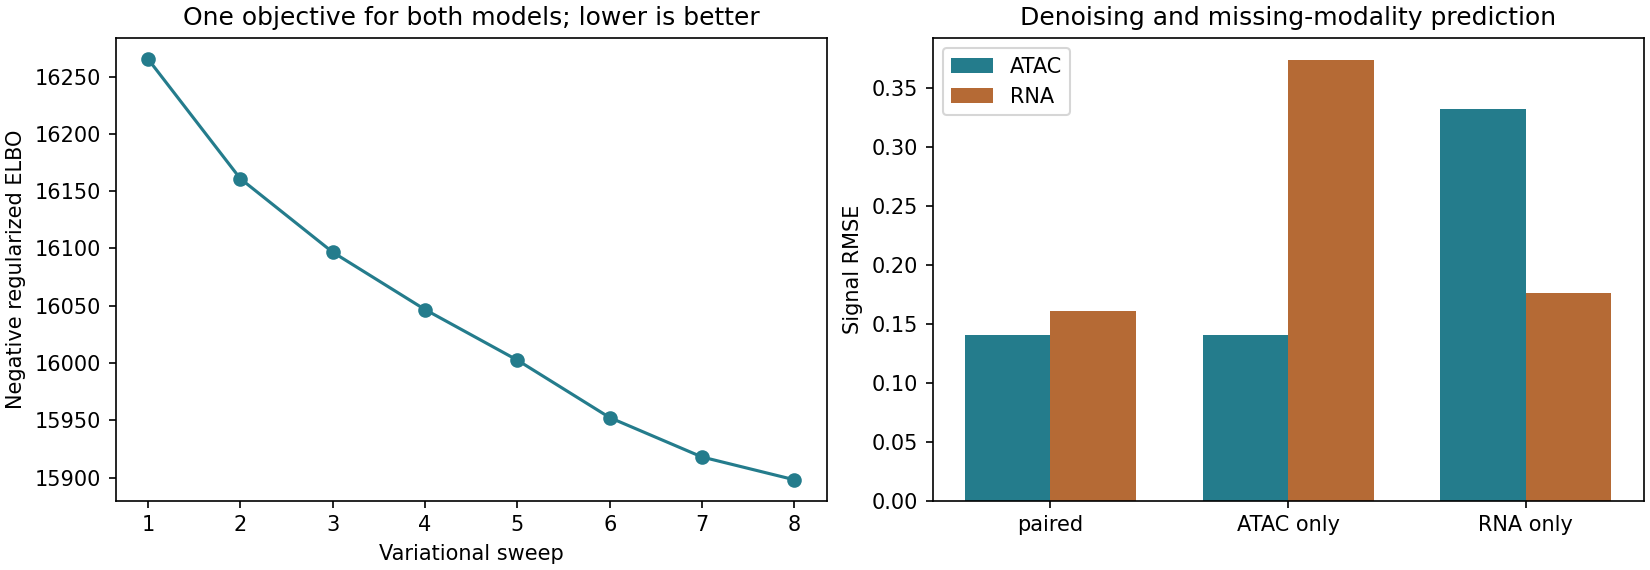
\includegraphics[width=\linewidth]{../atac_rna_joint/learning_and_errors.png}
\end{center}
The shared numerical objective decreased in this run. That observation is
not an unconditional convergence guarantee. Run the notebook from top to
bottom and increase integration resolution before drawing performance
conclusions. The revised short example completed in about 22 seconds in the tested
CPU environment with one torch thread; this is not a cross-method timing
benchmark.

\clearpage
\clearpage
\section{Adversarial numerical review and device handling}
\label{sec:numerical-audit}
\textit{Review added 16 September 2026.} The target remains
\(p(L_k\mid L_{<k})\). Removing latent-covariate edges gives the same
normal-means empirical Bayes subproblem; the implementation dispatches this
case to the ordinary cEBMF solver. This algebraic statement does not assert
that every finite neural optimization attains the subproblem optimum.

\subsection{A correct formula can be an unstable implementation}
Completing a Gaussian square using its natural parameters subtracts terms
of order \(\mu^2/s^2\). In float32 this failed for a prior with spike weight
0.2 and slab \(\N(10,10^{-8})\), with likelihood statistics \(a=2,b=3\).
The old numerical profile returned a posterior mean near 0.0125; the
independent analytic posterior is approximately \(1.59\times10^{-29}\).
This is cancellation error, not Monte Carlo variability.

For each continuous component, compute instead
\begin{align}
t&=\E[s(P)^{-2}], &
c&=\frac{\E[\mu(P)s(P)^{-2}]}{t},\\
h&=\E\log\pi(P)-\frac12\E\!\left[
 \log(2\pi s(P)^2)+\frac{(\mu(P)-c)^2}{s(P)^2}\right].
\end{align}
Then the expected log prior is exactly
\[
A(v)=h-\tfrac12t(v-c)^2.
\]
The spread in this expression is evaluated as an average of squared
centered differences, never as a difference of large second moments.
The height \(h\) retains the parameter-dependent normalization of
\(\exp(\E\log g)\); dropping it would change empirical Bayes learning.

Write \(\alpha=a+t\), \(r=t/\alpha\). The likelihood-completed Gaussian
has mean \(m=rc+b/\alpha\), variance \(V=1/\alpha\), and log mass
\begin{equation}
B=h+r(-ac^2/2+bc)+\frac{b^2}{2\alpha}
  +\frac12\log\frac{2\pi}{\alpha}.
\end{equation}
Its tilted contribution is \(\exp(B)\E_{N(m,V)}\exp D(v)\).
For the zero atom the corresponding log mass before the child tilt is
\(\E\log\pi_0(P)\). These are algebraic rearrangements of the earlier
derivation, not a different statistical model.

At a standard-normal quadrature node \(x_j\), evaluate the slab log density
as \(-\tfrac12\{\log(2\pi V)+x_j^2\}\). Combining it with \(B+D(v)-\log Z\)
gives the continuous-and-label log posterior used for entropy. This avoids
another unstable natural-parameter polynomial. For child feedback use
\[
\E[(L_c-\mu(P))^2\mid Z_c=h]
=\operatorname{Var}(L_c\mid Z_c=h)
 +(\E[L_c\mid Z_c=h]-\mu(P))^2,
\]
computing the within-component variance directly from centered nodes.

\subsection{What was checked, and what was not established}
Independent checks include exhaustive binary enumeration, analytic mixture
posteriors (including zero likelihood precision), and a dense trapezoidal
integral for a nonlinear logistic child tilt. Evidence, moments, entropy,
and parameter gradients agree at the stated test tolerances. Direct child
integration also checks the sparsity penalty and missing-branch mask.
The ordinary spike--normal posterior now uses log-domain component odds;
normal-mixture likelihoods are no longer silently clipped in the tails.

These tests do not prove convergence of finite quadrature for every neural
prior. Multiple-parent expectations use a finite fixed Sobol approximation;
the stored quadrature representation also approximates each continuous
coordinate. Local profile checkpoint selection is not a proof of global
ELBO ascent under those approximations. The posterior is still factorized
across loading coordinates. Better prior flexibility can lose predictive
accuracy through optimization, approximation, or overfitting.

The saved tree benchmark predates these numerical fixes. Inspecting its
checkpoints confirms float32 observations and loadings; the earlier claim
of float64 fitting was incorrect. The narrow-slab bug could affect those
fits, but attributing the performance gap to it requires matched reruns.
Original source hashes and measurements are retained and have not been
relabeled as results of the revised implementation.

\subsection{CUDA contract and its validation limit}
Loading moments, networks, quadrature states, optimizer state, residuals,
and objective histories are kept on the selected device. Conditional
checkpoint selection and mixture-EM convergence use device tensors.
Observation indices and prediction tables are cached. Sobol tables are
constructed once on CPU and transferred at graph setup. Ordinary CUDA
neural solvers batch with device indices.

ASH's automatically sized scale grid needs one host scalar for its length;
its amplitudes stay on device. Supplying a fixed \texttt{scales} tensor to
the ash prior removes that dynamic-size decision and still refits weights
on every sweep. Fixed-grid choice is a modeling choice, not an automatically
equivalent replacement for an adaptive grid. Rank pruning, boundary input
validation, plotting, and explicit reporting may also synchronize.

The development environment has PyTorch 2.11.0+cpu and no CUDA runtime.
CUDA-only tests cover complete warmed sweeps, partially paired modalities,
optimizer-state residency, CPU/GPU numerical agreement, profiler transfers,
and retained memory. They are skipped here, not reported as GPU passes.
Hardware validation remains required before making a measured GPU speed or
memory claim. The deprecated experimental sampler and optional L-BFGS route
are outside the synchronization-free conditional/ash-EM contract.


\begin{thebibliography}{99}\small
\bibitem{wang} W. Wang and M. Stephens (2021). Empirical Bayes Matrix
Factorization. \emph{JMLR} 22(120). \url{https://www.jmlr.org/papers/v22/20-589.html}.
\bibitem{cebmf} W. R. P. Denault et al. (2025). Covariate-moderated Empirical
Bayes Matrix Factorization. \url{https://arxiv.org/abs/2505.11639v2}.
\bibitem{twineb} S. Salehi, A. Nazaret, S. P. Shah and D. M. Blei (2024).
Population Priors for Matrix Factorization. \emph{TMLR}.
\url{https://openreview.net/forum?id=AT9G5s1p0j}.
\bibitem{vampprior} J. M. Tomczak and M. Welling (2018). VAE with a VampPrior.
\emph{AISTATS}, PMLR 84. \url{https://proceedings.mlr.press/v84/tomczak18a.html}.
\bibitem{vlae} X. Chen et al. (2017). Variational Lossy Autoencoder.
\url{https://arxiv.org/abs/1611.02731}.
\bibitem{ivae} I. Khemakhem, D. P. Kingma, R. P. Monti and A. Hyv\"arinen
(2020). Variational Autoencoders and Nonlinear ICA: A Unifying Framework.
\emph{AISTATS}, PMLR 108. \url{https://proceedings.mlr.press/v108/khemakhem20a.html}.
\bibitem{mofa} R. Argelaguet et al. (2020). MOFA+: a statistical framework for
comprehensive integration of multi-modal single-cell data.
\emph{Genome Biology} 21, 111. \url{https://doi.org/10.1186/s13059-020-02015-1}.
\bibitem{jive} E. F. Lock et al. (2013). Joint and Individual Variation
Explained (JIVE) for integrated analysis of multiple data types.
\emph{Annals of Applied Statistics} 7, 523--542.
\url{https://pmc.ncbi.nlm.nih.gov/articles/PMC3671601/}.
\bibitem{cavachon} Hsieh et al. (2024). CAVACHON: a hierarchical variational
autoencoder to integrate multi-modal single-cell data.
\url{https://arxiv.org/abs/2405.18655}.
\bibitem{multivi} T. Ashuach et al. (2023). MultiVI: deep generative model
for the integration of multimodal data. \emph{Nature Methods}.
\url{https://www.nature.com/articles/s41592-023-01909-9}.
\bibitem{glue} Z. J. Cao and G. Gao (2022). Multi-omics single-cell data
integration and regulatory inference with graph-linked embedding.
\emph{Nature Biotechnology}.
\url{https://pmc.ncbi.nlm.nih.gov/articles/PMC9546775/}.
\end{thebibliography}
\end{document}
